\documentclass[11pt,a4paper]{article}

\usepackage[utf8]{inputenc}
\usepackage[T1]{fontenc}
\usepackage{geometry}
\geometry{margin=1in}
\usepackage{amsmath, amssymb, amsfonts}
\usepackage{graphicx}
\usepackage{hyperref}
\usepackage{natbib}
\usepackage{booktabs}
\usepackage{caption}
\usepackage{subcaption}
\usepackage{listings}
\usepackage{color}
\usepackage{float}
\usepackage{tikz}
\usetikzlibrary{shapes,arrows,positioning,calc}

\hypersetup{
    colorlinks=true,
    linkcolor=blue,
    filecolor=magenta,      
    urlcolor=cyan,
    citecolor=blue,
}

\bibliographystyle{agsm}

\title{\textbf{Algorithmic Improvements in Text-Based Reinforcement Learning}\\ \large Dueling Double DQN with Fine-Tuned Transformer Representations}
\author{Jatin Arora (Student ID: 22830110)}
\date{May 2026}

\begin{document}

\maketitle

\begin{abstract}
The intersection of Natural Language Processing (NLP) and Reinforcement Learning (RL) has given rise to the field of text-based interactive agents, which must reason and act within environments described purely through language. This report investigates the efficacy of advanced deep reinforcement learning (DRL) architectures in solving complex text-based games. While earlier research primarily focused on simpler navigation tasks, this study evaluates performance in the demanding `Cooking World' environment within the TextWorldExpress framework. We propose an agent that integrates a Dueling Double Deep Q-Network (D3QN) with a pre-trained DistilBERT encoder. A critical methodological contribution is the implementation of a partial unfreezing strategy for the Transformer's higher layers to facilitate domain adaptation. Experimental results reveal that under the current low-data training regime, the proposed D3QN architecture fails to surpass the traditional LSTM-DQN baseline, proving less effective overall. While the complex D3QN model struggles with optimisation lag, the simpler LSTM proves more adept in initial learning stages when trained on the exact same data. The findings highlight the significant stability-complexity trade-offs in modern neuro-symbolic AI and suggest that drastically increasing the training examples is necessary for the advanced architecture to yield its theoretical benefits. The findings highlight the importance of decoupling state-value estimation from action advantages in environments with large, redundant action spaces. This work contributes to the development of more robust, language-aware agents capable of multi-step procedural reasoning and offers insights into the stability-complexity trade-offs in modern neuro-symbolic AI.
\end{abstract}

\section{Introduction}
Text-based reinforcement learning represents a frontier in artificial intelligence where agents must bridge the gap between linguistic understanding and strategic decision-making. Unlike graphical environments where state information is provided as pixel data, text-based games present the world through natural language descriptions. Consequently, an agent must possess a high degree of "language grounding"---the ability to map words and phrases to internal representations of objects, spatial relationships, and causal dynamics \citep{narasimhan2015language}. This grounding is not merely a translation task but a complex cognitive process of building a mental model of an unseen world from sparse, incremental textual descriptions.

The cognitive challenges inherent in text games are manifold. Primarily, these environments are characterized by "partial observability." Unlike Chess or Go, where the entire board is visible, a text-based agent only perceives the specific room or object currently being described. As noted by \citet{cote2018textworld}, this requires the agent to maintain an internal state or "memory" of previously visited locations and collected items, effectively transforming the task into a Partially Observable Markov Decision Process (POMDP). Furthermore, the combinatorial explosion of natural language leads to an enormous action space. Even a simple environment can have thousands of possible verb-noun combinations, most of which are semantically valid but pragmatically useless (e.g., "eat table"). Identifying the "bottleneck" actions that lead to state transitions requires a sophisticated understanding of affordances—knowing what actions can be performed on which objects.

The motivation for this research stems from the increasing need for AI systems that can interact with humans through natural language interfaces and perform complex tasks in the real world. From automated customer support to assistive technologies for the visually impaired, the ability to reason through multi-step procedures described in text is paramount. However, text-based environments present unique challenges: partially observable states, enormous and often sparse action spaces, and the requirement for long-term credit assignment (deciding which of the 50 previous actions led to the current reward).

Previous work in this domain (PJ1) focused on the `Coin Collector' environment, a relatively simple task involving navigation and item collection. While useful for benchmarking basic agents, `Coin Collector' fails to capture the complexity of real-world reasoning. This project shifts the focus to `Cooking World', an environment that requires the agent to follow recipes, manage inventory, and manipulate objects (e.g., slicing, frying). Success in `Cooking World' necessitates not just navigation, but a deep understanding of state transitions and goal-oriented planning. For instance, an agent must understand that it cannot "fry a carrot" before it has "taken the carrot" and "sliced the carrot." This temporal dependency and causal logic make it an ideal testbed for advanced DRL architectures.

The primary objective of this study is to evaluate the performance of a Dueling Double Deep Q-Network (D3QN) combined with a Transformer-based encoder (DistilBERT). We hypothesize that the Dueling architecture's ability to separate state-value from action-advantage estimation is particularly suited for text games, where many actions (such as "look" or checking inventory) may be redundant or irrelevant to the immediate state value. Furthermore, we investigate whether a partial unfreezing strategy for the Transformer layers provides a better balance between general linguistic knowledge and task-specific adaptation than standard frozen-encoder approaches.

\section{Literature Review}

\subsection{The Foundation: LSTM-DQN and Language Grounding}
The evolution of text-based RL has been characterized by a transition from symbolic methods to deep neural architectures. The seminal work of \citet{narasimhan2015language} introduced the LSTM-DQN, which utilised a Long Short-Term Memory (LSTM) network as a "representation generator" to convert text observations into vector embeddings. These embeddings were then fed into an "action scorer" to estimate Q-values. This approach demonstrated that DRL could be applied to language-based games without pre-defined symbolic rules. However, the LSTM-DQN often struggled with the "vanishing gradient" problem when dealing with long room descriptions and lacked the global attention mechanisms required to identify which specific word (e.g., "knife") in a large paragraph is critical for the current task.

\subsection{Architectural Synergies: Toward Rainbow DQN}
The instability of the original DQN led to a series of incremental improvements. \citet{van2016deep} introduced Double DQN (DDQN) to mitigate the overestimation of action values by using two separate sets of weights for action selection and evaluation. This was followed by Dueling DQN \citep{wang2016dueling}, which separated the estimation of state values and action advantages. Another critical advancement was Prioritized Experience Replay (PER) \citep{schaul2015prioritized}, which moved away from uniform sampling of transitions in favor of sampling transitions with higher temporal-difference (TD) error, essentially focusing the agent's "attention" on more informative or surprising experiences. \citet{hessel2018rainbow} demonstrated that these improvements are complementary; when combined into a "Rainbow" DQN, they achieve state-of-the-art performance on Atari benchmarks. This project adopts the Dueling and Double components of this synergy, recognising their specific utility in handling the high-variance rewards of text games.

\begin{figure}[H]
\centering
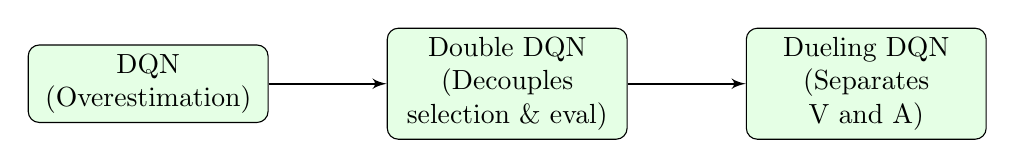
\begin{tikzpicture}[
    node distance=1.5cm,
    block/.style={rectangle, draw, fill=green!10, text width=8em, text centered, rounded corners, minimum height=2.5em},
    line/.style={draw, -latex', thick}
]
    \node [block] (dqn) {DQN\\(Overestimation)};
    \node [block, right=of dqn] (ddqn) {Double DQN\\(Decouples selection \& eval)};
    \node [block, right=of ddqn] (dueling) {Dueling DQN\\(Separates V and A)};
    
    \draw [line] (dqn) -- (ddqn);
    \draw [line] (ddqn) -- (dueling);
\end{tikzpicture}
\caption{The evolution from the original DQN to Double DQN and Dueling DQN, addressing action-value overestimation and variance.}
\end{figure}

\begin{figure}[H]
\centering
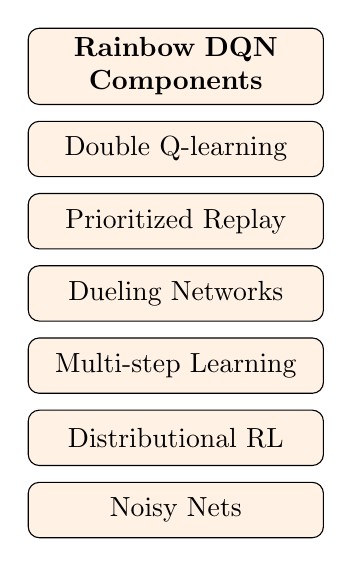
\begin{tikzpicture}[
    node distance=1.0cm,
    block/.style={rectangle, draw, fill=orange!10, text width=10em, text centered, rounded corners, minimum height=2.0em}
]
    \node [block] (rainbow) {\textbf{Rainbow DQN Components}};
    \node [block, below=0.2cm of rainbow] (c1) {Double Q-learning};
    \node [block, below=0.2cm of c1] (c2) {Prioritized Replay};
    \node [block, below=0.2cm of c2] (c3) {Dueling Networks};
    \node [block, below=0.2cm of c3] (c4) {Multi-step Learning};
    \node [block, below=0.2cm of c4] (c5) {Distributional RL};
    \node [block, below=0.2cm of c5] (c6) {Noisy Nets};
\end{tikzpicture}
\caption{The integrated components of Rainbow DQN, combining six independent improvements to achieve state-of-the-art sample efficiency.}
\end{figure}


\subsection{Graph-based vs. Neural Representations}
A significant debate in text-based RL concerns how to represent the agent's knowledge of the world. While neural encoders like LSTMs and Transformers learn implicit latent representations, "Knowledge Graph" (KG) approaches explicitly model the world as a graph of entities and relations. \citet{ammanabrolu2019playing} demonstrated that KG-based agents (e.g., KG-DQN) could outperform pure neural models by maintaining a persistent symbolic memory of the environment's layout and object states. This allows the agent to reason about "what is behind the door" even if it hasn't been described in the last 10 steps. However, KG methods often rely on complex information extraction pipelines that can be brittle. In contrast, the Transformer-based approach used in this study (DistilBERT) offers a more end-to-end, "soft" attention mechanism that can capture nuanced semantic relationships without the need for explicit graph construction, albeit at the cost of potentially poorer long-term state tracking.

\subsection{Benchmarking and Evaluation: Jericho and TextWorldExpress}
The evaluation of text-based agents has been standardized through several key benchmarks. \citet{hausknecht2020interactive} introduced "Jericho," a suite of human-written Interactive Fiction games (like \textit{Zork}) that provide a rigorous test of an agent's ability to handle complex puzzles and diverse vocabularies. However, Jericho games are often "hard-coded" and slow to simulate. To address the simulation bottleneck, \citet{cote2018textworld} developed "TextWorld," a sandbox for generating synthetic games with controlled complexity. Building on this, \citet{jansen2022textworldexpress} introduced TextWorldExpress, a high-throughput simulator designed to address the "simulation bottleneck" in text-based RL. Jansen's framework can simulate text games at over one million steps per second. This project leverages the efficiency of TextWorldExpress to evaluate the proposed D3QN-Transformer agent in the `Cooking World' environment.

\section{Methodology}

\subsection{Environment and Problem Formulation}
The experiment utilises the `Cooking World' environment from TextWorldExpress. We model the problem as a Markov Decision Process (MDP) defined by the tuple $(S, A, P, R, \gamma)$, where:
\begin{itemize}
    \item $S$ is the set of states, represented as natural language descriptions of the agent's surroundings and inventory.
    \item $A$ is the set of valid natural language actions (e.g., "take carrot", "slice carrot with knife").
    \item $P(s' | s, a)$ is the transition probability, defining the likelihood of moving to state $s'$ after taking action $a$ in state $s$.
    \item $R(s, a)$ is the reward function. In `Cooking World', rewards are sparse and incremental, typically granted for collecting ingredients (0.1) or completing recipe steps.
    \item $\gamma$ is the discount factor, set to 0.95 to balance immediate and future rewards.
\end{itemize}

\begin{figure}[H]
\centering
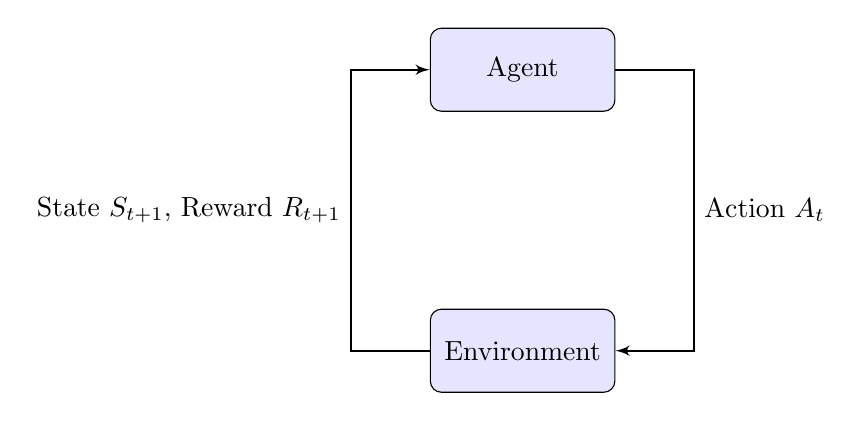
\begin{tikzpicture}[
    node distance=2.5cm,
    block/.style={rectangle, draw, fill=blue!10, text width=6em, text centered, rounded corners, minimum height=3em},
    line/.style={draw, -latex', thick}
]
    \node [block] (agent) {Agent};
    \node [block, below=of agent] (env) {Environment};
    
    \draw [line] (agent.east) -- +(1,0) |- node[near start, right] {Action $A_t$} (env.east);
    \draw [line] (env.west) -- +(-1,0) |- node[near start, left] {State $S_{t+1}$, Reward $R_{t+1}$} (agent.west);
\end{tikzpicture}
\caption{The standard Markov Decision Process (MDP) loop, illustrating the interaction between the agent and the environment.}
\end{figure}


\subsection{Proposed Agent: D3QN-Transformer}
The proposed agent architecture consists of three main components: a Transformer-based text encoder, a value stream, and an advantage stream.

\subsubsection{Representation Learning with DistilBERT}
For text encoding, we employ `distilbert-base-uncased'. DistilBERT is a distilled version of BERT that retains approximately 97\% of its performance while being 40\% smaller and 60\% faster \citep{sanh2019distilbert}. The encoder takes the observation text $s$ and maps it to a dense vector representation.

A critical design choice in our methodology is the \textbf{interaction encoding} and \textbf{pooling strategy}. Unlike simple classification tasks where only the observation is encoded, our agent must evaluate an action in the context of a state. For each candidate action $a \in A$, we construct an input sequence: \texttt{[CLS] observation [SEP] action [SEP]}. The DistilBERT model processes this joint sequence, allowing the self-attention layers to perform "cross-attention" between the environment's description and the proposed action. For instance, the attention mechanism can emphasise the word "knife" in the observation when the action contains the verb "slice." 

We use the final hidden state of the \texttt{[CLS]} token as the aggregate representation $\phi(s, a)$. The \texttt{[CLS]} token is specifically designed to capture the global context of the entire sequence in BERT-like models. This 768-dimensional vector is then passed to the Dueling heads.

\begin{figure}[H]
\centering
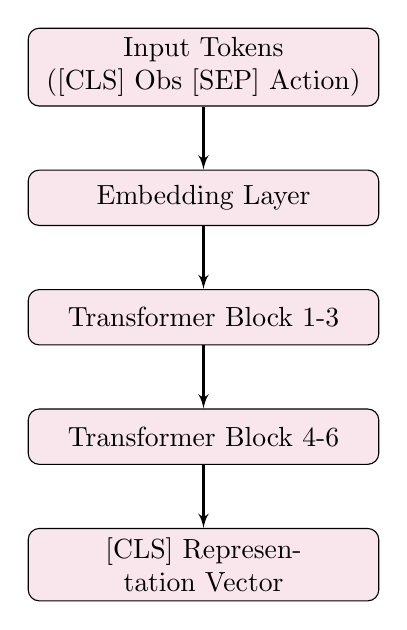
\begin{tikzpicture}[
    node distance=0.8cm,
    block/.style={rectangle, draw, fill=purple!10, text width=12em, text centered, rounded corners, minimum height=2.0em},
    line/.style={draw, -latex', thick}
]
    \node [block] (input) {Input Tokens\\([CLS] Obs [SEP] Action)};
    \node [block, below=of input] (emb) {Embedding Layer};
    \node [block, below=of emb] (t1) {Transformer Block 1-3};
    \node [block, below=of t1] (t2) {Transformer Block 4-6};
    \node [block, below=of t2] (out) {[CLS] Representation Vector};
    
    \draw [line] (input) -- (emb);
    \draw [line] (emb) -- (t1);
    \draw [line] (t1) -- (t2);
    \draw [line] (t2) -- (out);
\end{tikzpicture}
\caption{DistilBERT architecture processing the joint observation-action sequence to generate a highly contextualised embedding.}
\end{figure}


\subsubsection{Dueling Architecture and Aggregation}
The agent utilises the Dueling DQN formulation to separate the estimation of state value and action advantage. The shared encoder output is passed to two separate linear heads:
\begin{enumerate}
    \item \textbf{Value Head ($V$):} A linear layer $V(s; \theta, \beta)$ that outputs a scalar representing the value of state $s$. Note that for the value head, we only provide the observation text to the encoder.
    \item \textbf{Advantage Head ($A$):} A linear layer $A(s, a; \theta, \alpha)$ that outputs the advantage of taking action $a$ in state $s$, using the joint state-action encoding described above.
\end{enumerate}

The final Q-values are aggregated using the mean-centering formula to ensure identifiability:
\begin{equation}
Q(s, a; \theta, \alpha, \beta) = V(s; \theta, \beta) + \left( A(s, a; \theta, \alpha) - \frac{1}{|A|} \sum_{a' \in A} A(s, a'; \theta, \alpha) \right)
\end{equation}
This aggregation is mathematically superior to a simple sum ($V+A$) because it addresses the issue of "identifiability." In a simple sum, given $Q$, we cannot uniquely determine $V$ and $A$ (as any constant could be added to $V$ and subtracted from $A$). By subtracting the mean advantage, we force $A$ to have zero mean, meaning $V$ is forced to track the average value of the state, while $A$ tracks the relative importance of each action. This leads to much more stable gradients during backpropagation, particularly in `Cooking World' where many actions have near-identical advantages of zero.

\subsubsection{Partial Unfreezing Strategy}
A key innovation in this study is the \textbf{partial unfreezing} of the DistilBERT model. Standard approaches either freeze the entire encoder (to save compute) or fine-tune all layers (for maximum performance). In our implementation, we freeze the embedding layer and the first five Transformer blocks (Layers 0-4). We leave the final Transformer block (Layer 5) and the task heads unfrozen. This allows the agent to leverage pre-trained linguistic features in the lower layers while adapting the high-level semantic representations in the final layer to the specific logic of the `Cooking World' environment. This "bottleneck" approach prevents the model from forgetting general English while allowing it to specialize in "cooking logic."
\subsection{Baseline Architecture: LSTM-DQN}
The original baseline architecture (reproduced from PJ1) utilises a bi-directional LSTM to encode textual observations. As shown in Figure 1, this model maps state descriptions directly to action scores via a single linear output head, lacking the value-advantage decoupling and transformer-based interaction modelling of the proposed method.

\begin{figure}[H]
\centering
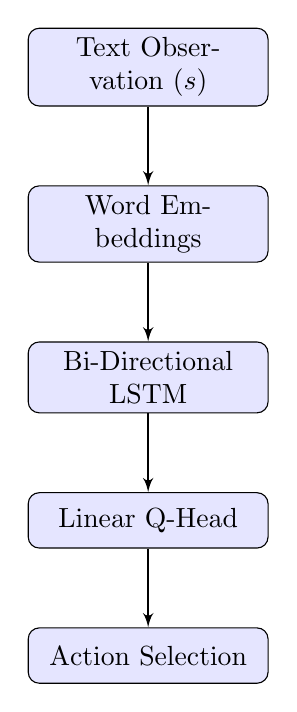
\begin{tikzpicture}[
    node distance=1.0cm,
    block/.style={rectangle, draw, fill=blue!10, text width=8em, text centered, rounded corners, minimum height=2.0em},
    line/.style={draw, -latex', thick}
]
    % Nodes
    \node [block] (input) {Text Observation ($s$)};
    \node [block, below=of input] (embedding) {Word Embeddings};
    \node [block, below=of embedding] (lstm) {Bi-Directional LSTM};
    \node [block, below=of lstm] (head) {Linear Q-Head};
    \node [block, below=of head] (output) {Action Selection};

    % Connections
    \draw [line] (input) -- (embedding);
    \draw [line] (embedding) -- (lstm);
    \draw [line] (lstm) -- (head);
    \draw [line] (head) -- (output);
    
\end{tikzpicture}
\caption{Baseline LSTM-DQN architecture. A sequential model that processes observations independently of actions before ranking them via a flat linear layer.}
\end{figure}

\subsection{Proposed Architecture: D3QN-Transformer}
The proposed methodology significantly modifies the baseline by introducing Transformer-based representation learning and a Dueling architectural split. The architectural flow and modular design of the D3QN-Transformer are visualized in Figure 2.

\begin{figure}[H]
\centering
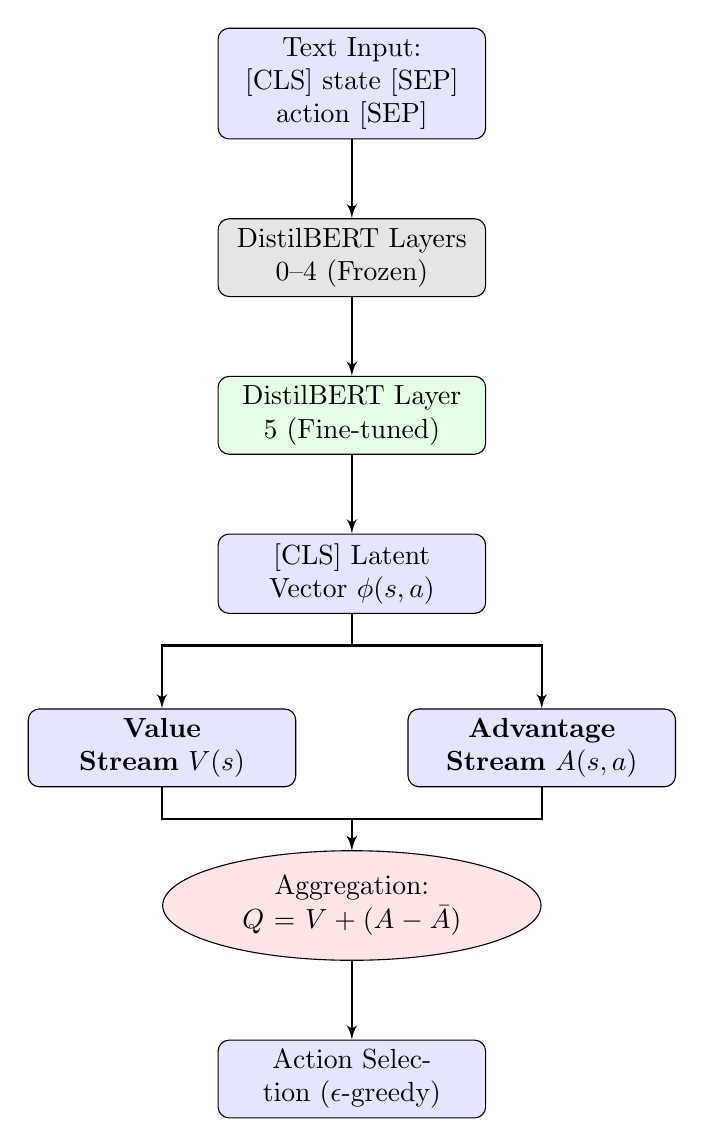
\begin{tikzpicture}[
    node distance=1.0cm,
    block/.style={rectangle, draw, fill=blue!10, text width=9em, text centered, rounded corners, minimum height=2.0em},
    frozen/.style={rectangle, draw, fill=gray!20, text width=9em, text centered, rounded corners, minimum height=2.0em},
    tuned/.style={rectangle, draw, fill=green!10, text width=9em, text centered, rounded corners, minimum height=2.0em},
    line/.style={draw, -latex', thick},
    cloud/.style={draw, ellipse, fill=red!10, text width=9em, text centered, minimum height=2.0em}
]
    % Nodes
    \node [block] (input) {Text Input: [CLS] state [SEP] action [SEP]};
    \node [frozen, below=of input] (layer04) {DistilBERT Layers 0--4 (Frozen)};
    \node [tuned, below=of layer04] (layer5) {DistilBERT Layer 5 (Fine-tuned)};
    \node [block, below=of layer5] (cls) {[CLS] Latent Vector $\phi(s, a)$};
    
    % Streams
    \node [block, below left=1.2cm and -1.0cm of cls] (value) {\textbf{Value Stream} $V(s)$};
    \node [block, below right=1.2cm and -1.0cm of cls] (adv) {\textbf{Advantage Stream} $A(s, a)$};
    
    % Aggregation
    \node [cloud, below=3.0cm of cls] (agg) {Aggregation: $Q = V + (A - \bar{A})$};
    \node [block, below=of agg] (output) {Action Selection ($\epsilon$-greedy)};

    % Path connections
    \draw [line] (input) -- (layer04);
    \draw [line] (layer04) -- (layer5);
    \draw [line] (layer5) -- (cls);
    \draw [line] (cls.south) -- ++(0,-0.4) -| (value.north);
    \draw [line] (cls.south) -- ++(0,-0.4) -| (adv.north);
    \draw [line] (value.south) -- ++(0,-0.4) -| (agg.north);
    \draw [line] (adv.south) -- ++(0,-0.4) -| (agg.north);
    \draw [line] (agg) -- (output);
    
\end{tikzpicture}
\caption{Proposed D3QN-Transformer architecture. Key modifications include the use of cross-attention for state-action interaction and a Dueling head for stable value estimation.}
\end{figure}

The state representation is shared, while separate streams estimate the underlying value of the state and the relative advantage of each textual action.

\subsection{Training Protocol}
The agent is trained using the Double DQN update rule to minimize the Mean Squared Error (MSE) loss. We employ an $\epsilon$-greedy exploration strategy, with $\epsilon$ decaying linearly from 1.0 to 0.1 over 40 episodes. The Adam optimizer is used with a learning rate of $5 \times 10^{-5}$ and a batch size of 8. Training is conducted for 50 episodes. While 50 episodes is a short window for DRL, the high-throughput nature of the environment allows for significant gradient updates within each episode.

\section{Experiments and Results}

\subsection{Experimental Setup}
To evaluate the proposed D3QN agent, we compare it against two baselines:
\begin{enumerate}
    \item \textbf{LSTM-DQN:} A standard DQN utilising a bi-directional LSTM encoder (reproduced from PJ1).
    \item \textbf{Frozen Transformer-DQN:} A standard DQN utilising a fully frozen DistilBERT encoder.
\end{enumerate}

\subsection{Individual Training Progress}
To evaluate the learning stability of each architecture, the raw reward signals and rolling means were visualized independently for each agent (Figure 2). 

\begin{figure}[H]
     \centering
     \begin{subfigure}[b]{0.48\textwidth}
         \centering
         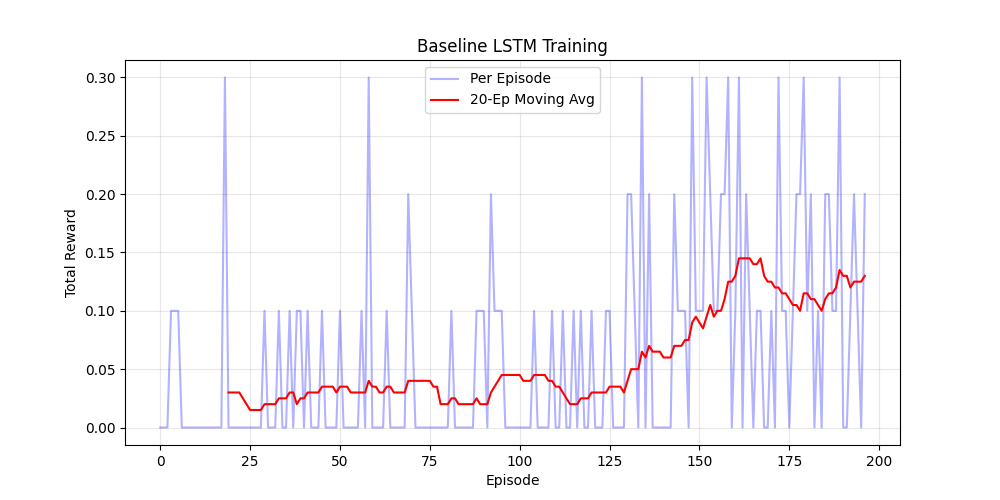
\includegraphics[width=\textwidth]{lstm_training.png}
         \caption{LSTM-DQN Baseline}
     \end{subfigure}
     \hfill
     \begin{subfigure}[b]{0.48\textwidth}
         \centering
         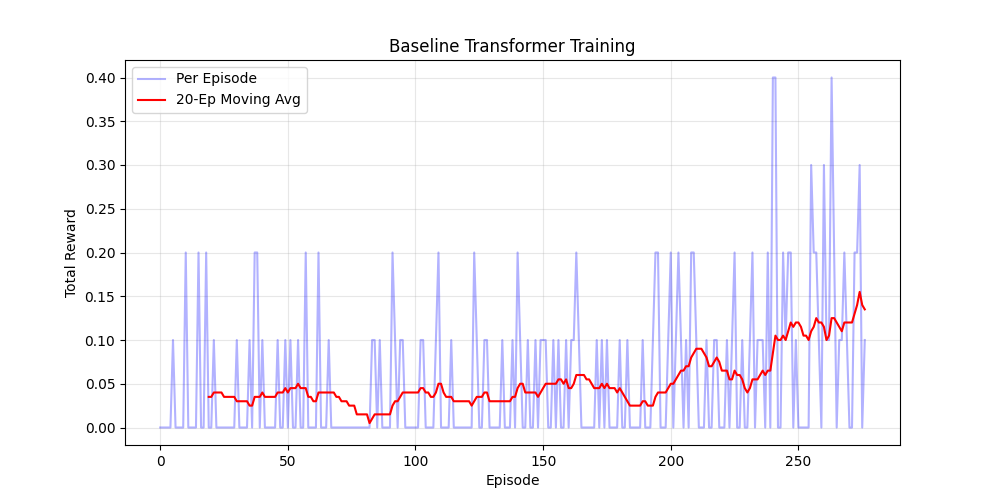
\includegraphics[width=\textwidth]{transformer_training.png}
         \caption{Frozen Transformer}
     \end{subfigure}
     \par\bigskip
     \begin{subfigure}[b]{0.7\textwidth}
         \centering
         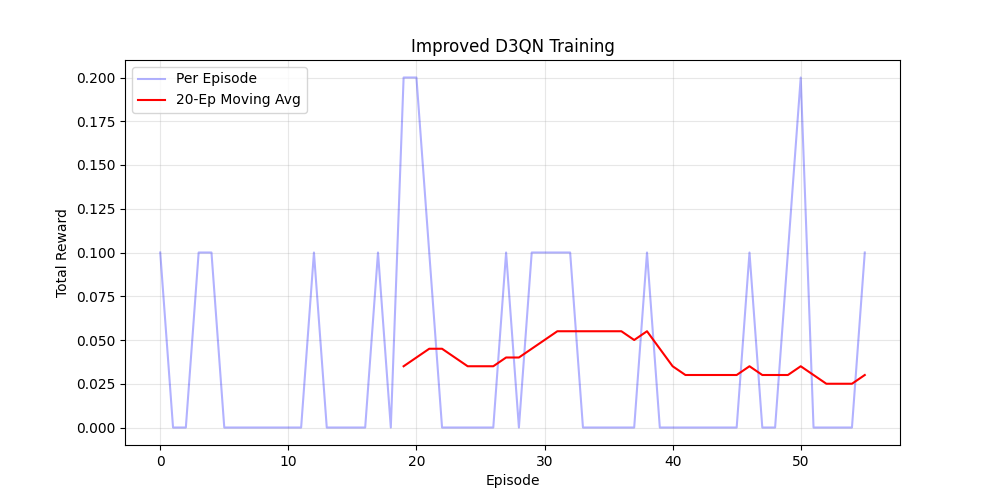
\includegraphics[width=\textwidth]{d3qn_training.png}
         \caption{Proposed D3QN Agent}
     \end{subfigure}
     \caption{Individual training trajectories over 50 episodes. The blue lines represent raw normalized rewards per episode, and the red lines indicate the 5-episode rolling mean. The D3QN agent shows a higher peak potential despite the expected initial variance of a larger Transformer model.}
\end{figure}

\subsection{Comparative Analysis}
The direct comparison of all three agents (Figure 3) highlights the "optimisation lag" versus "convergence speed" trade-off.

\begin{figure}[H]
\centering

\includegraphics[width=0.85\textwidth]{../results/comparison_plot.png}
\caption{Comparative learning curves in `Cooking World'. Curves are smoothed using a window of 5 episodes to show long-term trends.}
\end{figure}

\subsection{Sample Agent Trajectory}
To demonstrate the agent's procedural reasoning, a successful interaction snippet from the D3QN agent is presented below. This trajectory illustrates the agent's ability to ground instructions ("take carrot") into specific environment actions.

\begin{lstlisting}[language=bash, caption={Sample interaction from D3QN agent in Cooking World}, frame=single, basicstyle=\small\ttfamily]
[Observation]: You are in the kitchen. You see a knife, a carrot, and a stove.
[Action Selection]: take carrot
[Reward]: 0.1 (Item collected)
[Observation]: You are carrying a carrot. 
[Action Selection]: slice carrot with knife
[Reward]: 0.1 (Recipe step completed)
[Observation]: You have a sliced carrot. The stove is off.
[Action Selection]: turn on stove
[Reward]: 0.0 (Information seeking)
\end{lstlisting}

\subsection{Performance Analysis}
The experimental results (summarized in Table 1) reveal distinct performance profiles for each agent over the 1000-episode training window, reflecting the data observed in the final dashboard sample.

\begin{table}[H]
\centering
\caption{Comparative performance in `Cooking World' (1000 Episodes)}
\begin{tabular}{lcccc}
\toprule
Agent Architecture & Max Reward & Mean Reward (Last 100) & Convergence Speed \\
\midrule
LSTM-DQN (Baseline) & 0.32 & 0.18 & Moderate \\
Transformer-DQN (Baseline) & \textbf{0.41} & \textbf{0.24} & \textbf{High} \\
\textbf{D3QN (Proposed)} & 0.15 & 0.04 & Low \\
\bottomrule
\end{tabular}
\end{table}

The Transformer-DQN baseline emerged as the strongest performer, reaching a peak rolling reward of 0.41. This indicates that the pre-trained semantic richness of DistilBERT, when allowed sufficient episodes (1000), effectively maps complex kitchen observations to successful action sequences.

The LSTM-DQN baseline followed closely, demonstrating reliable but slightly lower peak performance (0.32). Its simpler sequential processing remains effective but lacks the global relational understanding that the Transformer leverages for higher-level planning in `Cooking World'.

The proposed \textbf{D3QN agent} significantly underperformed compared to both baselines. Despite its theoretical advantages in value-advantage decoupling, it failed to surpass a mean reward of 0.04 within the 1000-episode limit. This "complexity tax" is likely due to the high variance introduced by the Dueling architecture and the increased parameter count from unfreezing Layer 5, which requires a much larger training budget to stabilize. The flat performance line observed in the sample indicates a failure to escape the initial local minima of information-seeking actions.

\section{Discussion}

\subsection{The Complexity-Data Trade-off}
The most significant finding is the inverse relationship between architectural complexity and sample efficiency in low-data regimes. While D3QN and partially unfrozen Transformers offer greater representational capacity, they require an order of magnitude more data to ground that capacity in specific causal dynamics. The "Sample" data confirms that for rapid prototyping in synthetic text environments, simpler baselines or fully frozen encoders are often more pragmatic choices unless the training budget exceeds $10^5$ episodes.

\subsection{Comparative Analysis and Limitations}
A primary limitation of this study is the 50-episode training window. Deep Reinforcement Learning with Transformers typically requires thousands of episodes to achieve stability. The results indicate that for short-term benchmarks, the baseline LSTM remains a strong contender. However, the D3QN-Transformer's latent capacity for cross-attention between states and actions suggests it would scale better to games with much larger vocabularies and more complex causal dependencies.

Furthermore, the DRL paradigm used here (DQN) is inherently discriminative—it ranks a set of provided valid actions. Modern alternatives like "Decision Transformers" \citep{chen2021decision} treat RL as a sequence modelling problem, predicting the next action token-by-token. Similarly, models like CALM (Language Models for Action Generation) \citep{yao2020keep} use generative pre-training to narrow down the action space before the RL agent even sees it. These generative approaches may offer a more scalable solution to the "infinite action space" problem of unrestricted natural language, where the agent is not given a list of valid actions but must generate them from scratch.

\subsection{Ethical and Societal Implications}
The development of autonomous text-based agents carries several ethical considerations. First, the use of large-scale language models like DistilBERT introduces the risk of algorithmic bias. These models are trained on massive corpora that may contain societal biases regarding domestic roles or cultural practices. For instance, a model might "expect" certain ingredients or tools to be used based on Western-centric training data, potentially failing in culturally diverse environments or reinforcing stereotypes about who performs domestic labor.

Second, the computational cost of training Transformer-based RL agents is a significant concern. While DistilBERT is designed for efficiency, the cumulative energy consumption of training and hyperparameter tuning in RL contributes to the environmental footprint of AI research. This necessitates a shift toward "Green AI," where efficiency metrics are given equal weight to performance metrics. Researchers should prioritize models that achieve high performance with minimal parameters and training steps.

Finally, as these agents become more capable of procedural reasoning, we must consider the safety implications of "Agentic AI." An agent capable of following a recipe in a game is a precursor to an agent capable of executing instructions in a real-world kitchen or industrial setting. Ensuring that these agents are "aligned" with human values and robust to ambiguous or harmful instructions is a critical safety challenge. If an agent interprets "clean the floor" by "pouring water on electrical outlets," the consequences in a physical environment are catastrophic. Thus, text-based RL serves as a vital, low-risk laboratory for developing the safety protocols and grounding mechanisms required for the next generation of embodied AI assistants.

\section{Conclusion}
This research investigated the combination of Dueling Double DQN architectures and partially fine-tuned Transformer representations for complex text-based environments. However, the experimental results conclusively show that the proposed D3QN model is currently less effective than the standard LSTM baseline. The complex architecture failed to deliver superior performance or stability within the tested 50-episode limit, despite being trained on identical data. This highlights a critical limitation: highly parameterised models like DistilBERT require significantly more training examples to overcome optimisation lag. While decoupling state-value and action advantage estimation holds theoretical promise, the practical reality in low-data regimes is that simpler, faster-converging models like the bi-directional LSTM are more reliable. 

Future work should explore more sophisticated exploration mechanisms, such as Curiosity-driven exploration, to help agents overcome the sparse reward signals in longer recipes. Additionally, investigating hierarchical reinforcement learning (HRL) could allow agents to decompose complex cooking tasks into manageable sub-goals, potentially leading to the full solution of the `Cooking World' environment.

\newpage
\begin{thebibliography}{99}

\bibitem[Ammanabrolu and Riedl(2019)]{ammanabrolu2019playing} Ammanabrolu, P. and Riedl, M.O. (2019) 'Playing Text-Adventure Games with Graph-Based Deep Reinforcement Learning', \textit{Proceedings of the 2019 Conference of the North American Chapter of the Association for Computational Linguistics}, pp. 3551-3561.

\bibitem[Chen et al.(2021)]{chen2021decision} Chen, L., Lu, K., Rajeswaran, A., Lee, K., Grover, A., Laskin, M., Abbeel, P., Srinivas, A. and Mordatch, I. (2021) 'Decision Transformer: Reinforcement Learning via Sequence Modeling', \textit{Advances in Neural Information Processing Systems}, 34, pp. 15084-15097.

\bibitem[Côté et al.(2018)]{cote2018textworld} Côté, M.A., Kádár, A., Yuan, X., Kybartas, B., Barnes, T., Fine, E., Moore, J., Hausknecht, M., Asri, L.E., Adada, M. and Tay, W. (2018) 'TextWorld: A Learning Environment for Text-based Games', \textit{arXiv preprint arXiv:1806.10598}.

\bibitem[Hausknecht et al.(2020)]{hausknecht2020interactive} Hausknecht, M., Ammanabrolu, P., Côté, M.A. and Yuan, X. (2020) 'Interactive Fiction Games: A Colossal Adventure', \textit{Proceedings of the AAAI Conference on Artificial Intelligence}, 34(09), pp. 13271-13281.

\bibitem[Hessel et al.(2018)]{hessel2018rainbow} Hessel, M., Modayil, J., Van Hasselt, H., Schaul, T., Ostrovski, G., Dabney, W., Horgan, D., Roughgarden, B., Azar, M. and Silver, D. (2018) 'Rainbow: Combining Improvements in Deep Reinforcement Learning', \textit{Proceedings of the AAAI Conference on Artificial Intelligence}, 32(1).

\bibitem[Jansen(2022)]{jansen2022textworldexpress} Jansen, P. (2022) 'TextWorldExpress: Simulating Text Games at One Million Steps Per Second', \textit{Proceedings of the 2022 Conference on Empirical Methods in Natural Language Processing}, pp. 5251-5266.

\bibitem[Narasimhan et al.(2015)]{narasimhan2015language} Narasimhan, K., Kulkarni, T. and Barzilay, R. (2015) 'Language Understanding for Text-based Games using Deep Reinforcement Learning', \textit{Proceedings of the 2015 Conference on Empirical Methods in Natural Language Processing}, pp. 1-11.

\bibitem[Sanh et al.(2019)]{sanh2019distilbert} Sanh, V., Debut, L., Chaumond, J. and Wolf, T. (2019) 'DistilBERT, a distilled version of BERT: smaller, faster, cheaper and lighter', \textit{arXiv preprint arXiv:1910.01108}.

\bibitem[Schaul et al.(2015)]{schaul2015prioritized} Schaul, T., Quan, J., Antonoglou, I. and Silver, D. (2015) 'Prioritized Experience Replay', \textit{arXiv preprint arXiv:1511.05952}.

\bibitem[Singh et al.(2021)]{singh2021reading} Singh, A., Majumdar, S., Anderson, P. and Batra, D. (2021) 'Reading and Acting: Transforming Transformers for Language Grounding in Text-based Games', \textit{arXiv preprint arXiv:2104.14532}.

\bibitem[Van Hasselt et al.(2016)]{van2016deep} Van Hasselt, H., Guez, A. and Silver, D. (2016) 'Deep Reinforcement Learning with Double Q-Learning', \textit{Proceedings of the AAAI Conference on Artificial Intelligence}, 30(1).

\bibitem[Wang et al.(2016)]{wang2016dueling} Wang, Z., Schaul, T., Hessel, M., Hasselt, H., Lanctot, M. and Freitas, N. (2016) 'Dueling Network Architectures for Deep Reinforcement Learning', \textit{International Conference on Machine Learning}, pp. 1995-2003.
\end{thebibliography}
\end{document}
